\subsection{Descripción del algoritmo implementado. Podas y estrategias.}
\vspace*{0.3cm}

\textcolor{red}{\textbf{completar!}}

El algoritmo es un backtracking que recorre todos los nodos y todos los
conjuntos posibles y, recursivamente, se fija cual es mejor.  La única poda
consiste en cada iteración calcular si el peso actual de la partición es mayor
al peso de la partición mínima encontrada hasta ese momento y, de ser así,
cortar la recursión.


\newpage

\subsection{Análisis de complejidad en el peor caso.}
\vspace*{0.3cm}

En primer lugar, es necesario observar que, si $k > n$, la solución el problema
es distribuir los vértices en $n$ particiones, es decir, poner un vértice en
cada partición, obteniendo peso $0$ en total, pues no hay aristas
intrapartición. Luego, al no haber diferencia en la cantidad en la resolución
del problema si $k > n$ a si $k = n$ (salvo por la presencia de particiones
vacías), se asume $k \le n$.

Teniendo en cuenta esta observación, el algoritmo busca encontrar la
partición en $k$ subconjuntos \textit{no vacíos} los $n$ vértices del grafo,
asegurando que la sumatoria de los pesos de cada uno de los $k$ subconjuntos
sea mínima. Esto conlleva, en el peor de los casos, a buscar todos los posibles
modos de distribuir $n$ elementos distinguibles en $k$ conjunto distinguibles,
de modo tal que no haya elementos repetidos en los $k$ conjuntos. La cantidad
de particiones generadas coincide en este caso con el número de
Stirling\footnote{
\url{https://en.wikipedia.org/wiki/Stirling_numbers_of_the_second_kind}} $S(n,
k)$.

Esto se logra insertando de a uno los vértices del grafo en algún conjunto de
la $k$-partición. Por cada uno de los $k$ conjuntos, el procedimiento es el
siguiente:
\begin{itemize}
  \item se inserta en el conjunto, lo que toma $O(n)$, pues para insertar un
  vértice en un conjunto de la partición, se debe calcular el nuevo peso de
  dicho conjunto y en el peor de los casos, todos los vértices pertenecen al
  conjunto.
  \item se comprueba si quedan no quedan más vértices por agregar y, de ser
  así, si el peso de la partición actual es menor al peso de la mejor partición
  encontrada hasta el momento, se toma la partición actual como la mejor
  partición hasta el momento, realizando una copia de dicha partición, lo que
  toma $O(n)$, pues en el peor de los casos todos los vértices están
  distribuidos en los conjuntos de la $k$-partición.
  \item en caso contrario, se sigue con la recursión.
\end{itemize}

Luego, en la peor de las situaciones, la complejidad de cada paso de la
recursión es $O(n . k)$.

Esto se realiza hasta generar todas las posibles particiones en $k$ conjuntos.
Luego, la complejidad total del algoritmo es
\begin{align*}
  O(S(n, k) . n . k)
\end{align*}


\newpage \subsection{Experimentación y gráficos.}
\vspace*{0.3cm}

\subsubsection{Test algoritmo exacto}

(ver \verb|info.exacto.dat.promedio|) \medskip

Para realizar este test, se generaron aleatoriamente grafos de $n$ nodos, con  $n$ inicializado en 5 e incrementándose de a 1, hasta alcanzar 30 y $m$
(cantidad de aristas) vale $\frac{n^2}{5}$, $k$ vale $\frac{n}{3}$

Para cada instancia se toma el \textbf{valor mínimo}, medido en microsegundos, luego de \textbf{10 corridas}.

Dada una combinación de $m$, $n$ y $k$, se generaron 5 instancias aleatorias con dicha combinación y se consideró el promedio entre ellas.

\vspace*{0.5cm}

\begin{figure}[h]
  \begin{center}
    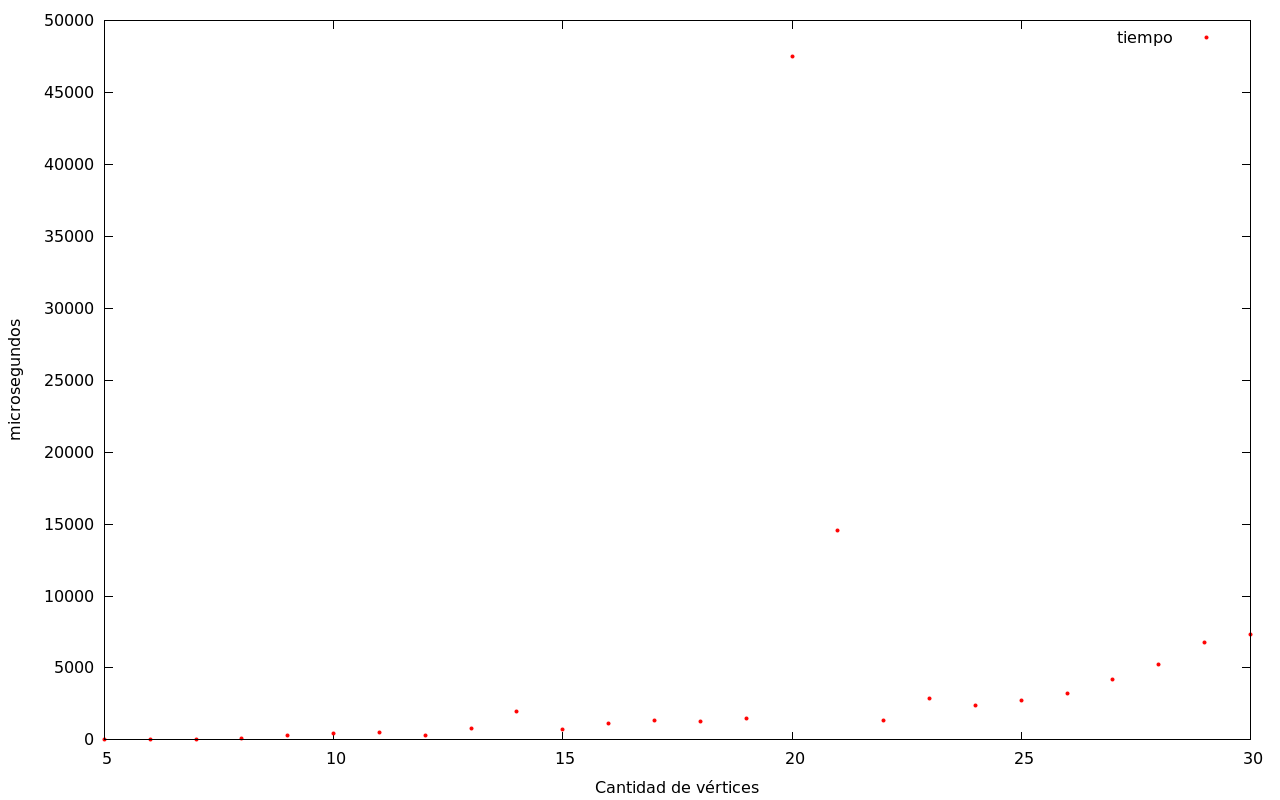
\includegraphics[scale=0.35]{imagenes/grafico-exacto.png}
  \end{center}
\end{figure}

\vspace*{0.5cm}

En el gráfico puede apreciarse que el algoritmo es \textit{``lento''}, lo cual era esperado debido a su naturaleza exponencial.
